\chapter{Resultados}

\section{Introdução aos Resultados}

Neste capítulo, os resultados obtidos a partir da aplicação dos métodos de classificação de texto analisados neste estudo são apresentados, incluindo tanto técnicas baseadas em Argmax quanto diversos métodos de aprendizado de máquina. A avaliação do desempenho desses métodos é considerada fundamental para compreender sua eficácia na classificação de descrições de produtos em português, utilizando o dataset RETAILPRODUCTDESCRIPTION-PTBR especialmente preparado para este fim.

Inicialmente, uma análise detalhada dos resultados obtidos com o método Argmax é apresentada, explorando diferentes configurações de vetorização, tokenização e normalização, e como estas são vistas para afetar o desempenho do método em termos de acurácia e F1-Score Macro.

Em seguida, procede-se à análise detalhada de cada método de aprendizado de máquina empregado neste estudo, incluindo SVM, Árvores de Decisão, Naive Bayes, k-Nearest Neighbors e Regressão Logística. Para cada um desses métodos, o capítulo inicia com a descrição do processo de ajuste fino (fine-tuning) dos hiperparâmetros, visando otimizar o desempenho em termos de acurácia e F1-Score Macro.

Após a fase de ajuste fino, os resultados gerais alcançados são apresentados, focando no desempenho otimizado de cada método e como as diferentes configurações impactam esse desempenho.

Finalmente, uma comparação geral dos resultados de todos os métodos analisados é realizada, oferecendo uma visão integrada do desempenho relativo de cada técnica. Esta seção de resultados gerais visa identificar os métodos mais promissores para a classificação de textos curtos em português, considerando as particularidades do dataset em estudo. Discussões sobre as limitações dos resultados, considerações para a interpretação dos dados e sugestões para pesquisas futuras também são abordadas, fornecendo um panorama completo dos achados e sua implicação para o campo do processamento de linguagem natural e aprendizado de máquina.

\subsection{Avaliação do Método Argmax}

Para a avaliação do método Argmax, diversas combinações de parâmetros foram examinadas. O foco desta análise reside na determinação de configurações ótimas que apresentam a melhor combinação de acurácia e f1score macro na tarefa de classificação de textos curto, especificamente nas descrições de produtos em português. As combinações de parâmetros selecionadas para estudo incluem:

As combinações de parâmetros selecionadas para o estudo foram:

\begin{itemize}
    \item \textbf{Método de Vetorização:} Foram consideradas abordagens binárias, frequência de termos (TF) e frequência de termos ponderada pelo inverso da frequência dos termos nos documentos (TF-IDF).
    \item \textbf{N-Gramas:} Unigramas (1,1) e unigramas com bigramas (1,2) foram avaliados.
    \item \textbf{Normalização:} A influência da normalização L2 foi examinada em comparação com a ausência de normalização.
\end{itemize}

Para uma compreensão completa do desempenho e da eficácia das diferentes configurações avaliadas, a análise será iniciada examinando os resultados das medidas de acurácia e F1 Score Macro para todas as combinações de parâmetros. Uma tabela detalhada será apresentada, incluindo o ranqueamento de cada método em cada medida, proporcionando uma visão abrangente do desempenho relativo de cada configuração. Em seguida, boxplots serão utilizados para visualizar a distribuição das medidas de acurácia e F1 Score Macro, destacando possíveis padrões e variações entre as configurações. Complementando esta análise, um gráfico bidimensional, denominado "Gráfico de Desempenho", será apresentado, ilustrando a relação entre acurácia (eixo x) e F1 Score Macro (eixo y) para cada configuração avaliada. Posteriormente, uma análise detalhada do impacto da tokenização e normalização em cada método será conduzida, identificando as configurações mais promissoras e destacando os pontos fortes e fracos de cada abordagem. Por fim, com base nos insights obtidos, recomendações serão oferecidas sobre as melhores práticas para a seleção de parâmetros e a configuração ideal do método Argmax em tarefas de classificação de texto em português.

\subsubsection{Resultados}

    Foram realizadas simulações com todas as combinações utilizando para testre e treino o método K-Fold com 10 partições.  Isto permite gerar estatísticas e avaliar a variância do método, aqui avaliada em porcentagem pelo coeficiente de variação.  A tabela \ref{tab:resultadoargmax_rankings} apresenta estas estatísticas.

\begin{table}[H]
\centering
\caption{Resultados estatísticos dos testes para o método Argmax com Rankings}
\label{tab:resultadoargmax_rankings}
\footnotesize % Diminui a fonte da tabela
\begin{tabular}{lllrrrrrr}
\hline
Método & NGram & Norm & \multicolumn{3}{c}{Acurácia (\%)} & \multicolumn{3}{c}{F1 Score Macro(\%)} \\
& & & Média & CV & \# & Média & CV & \# \\
\hline
Binary & [1, 1] & None & 75.31 & 0.44 & 6 & 58.77 & 3.15 & 3 \\
Binary & [1, 1] & L2 & 19.07 & 2.40 & 12 & 25.39 & 2.04 & 11 \\
Binary & [1, 2] & None & 89.56 & 0.21 & 1 & 70.09 & 1.91 & 1 \\
Binary & [1, 2] & L2 & 31.30 & 1.48 & 11 & 33.82 & 1.77 & 8 \\
TermFrequency & [1, 1] & None & 63.76 & 0.41 & 10 & 23.44 & 2.05 & 12 \\
TermFrequency & [1, 1] & L2 & 77.05 & 0.24 & 4 & 52.31 & 2.46 & 5 \\
TermFrequency & [1, 2] & None & 66.68 & 0.28 & 9 & 27.08 & 1.69 & 10 \\
TermFrequency & [1, 2] & L2 & 79.65 & 0.29 & 3 & 55.56 & 2.61 & 4 \\
TFIDF & [1, 1] & None & 70.64 & 0.28 & 8 & 32.10 & 2.25 & 9 \\
TFIDF & [1, 1] & L2 & 78.37 & 0.32 & 5 & 55.20 & 2.47 & 6 \\
TFIDF & [1, 2] & None & 74.57 & 0.33 & 7 & 37.67 & 1.53 & 7 \\
TFIDF & [1, 2] & L2 & 82.76 & 0.29 & 2 & 59.83 & 2.52 & 2 \\
\hline
\end{tabular}
\end{table}

\subsection{Análise dos Resultados}

\subsubsection{Acurácia}

Os resultados de acurácia revelam que o método Binary com NGram [1, 2] e sem normalização obteve a maior média de acurácia (89.56\%), seguido pelo método TFIDF com NGram [1, 2] e L2 (82.76\%). Por outro lado, o método Binary com NGram [1, 1] e L2 apresentou a menor média de acurácia (19.07\%). Observa-se que o método Binary com NGram [1, 1] e L2 apresentou o maior coeficiente de variação (CV) (2.40\%), indicando uma maior variabilidade nos resultados.

Os boxplots das acurácias (Figura \ref{fig:boxplot_acuracia}) demonstram uma variância relativamente baixa entre as combinações de parâmetros testadas. Observou-se a presença de poucos outliers, indicando que a maioria das configurações apresenta um desempenho consistente. As combinações que utilizam o método binário sem normalização destacaram-se por apresentar as melhores acurácias, enquanto aquelas com normalização L2 mostraram-se menos eficazes.
\begin{figure}[H]
    \centering
    \includegraphics[width=0.8\textwidth]{images/ArgmaxAcuráciaTodos.png}
    \caption{Boxplot das acurácias das combinações Argmax.}
    \label{fig:boxplot_acuracia}
\end{figure}

\subsubsection{F1 Score Macro}


Em relação ao F1 Score Macro, observa-se algumas diferenças em comparação com os resultados de acurácia. Por exemplo, o método Binary com NGram [1, 2] e sem normalização mantém sua posição de destaque, enquanto o método TFIDF com NGram [1, 1] e L2 apresenta um desempenho superior em relação ao método TermFrequency com a mesma configuração. As diferenças nos rankings atribuídos para acurácia e F1 Score destacam a importância de considerar múltiplas métricas ao avaliar o desempenho de modelos de classificação de texto.

Similarmente, os boxplots dos F1 Scores Macro (Figura \ref{fig:boxplot_f1score}) revelam que as configurações com bom desempenho em acurácia tendem também a exibir resultados satisfatórios no F1 Score Macro. Este padrão sugere que as configurações selecionadas são capazes de manter um equilíbrio razoável na performance entre as diversas classes, mesmo considerando o desbalanceamento presente no conjunto de dados.

\begin{figure}[H]
    \centering
    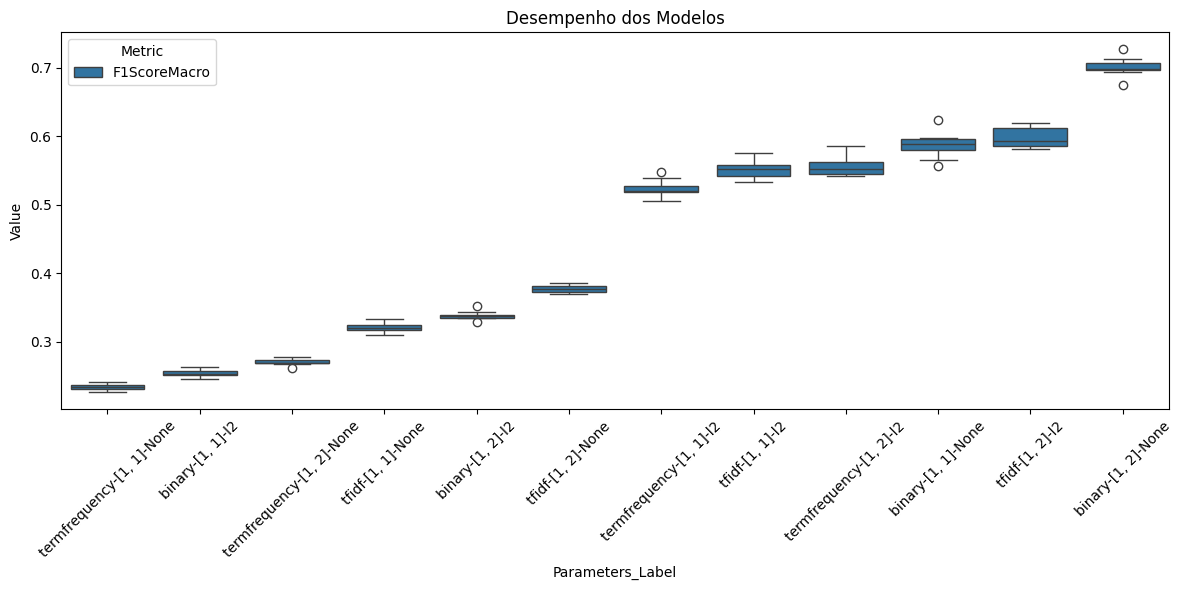
\includegraphics[width=0.8\textwidth]{images/ArgmaxF1ScoreTodos.png}
    \caption{Boxplot dos F1 Scores Macro das combinações Argmax.}
    \label{fig:boxplot_f1score}
\end{figure}

\subsubsection{Análise Combinada}

\subsection{Análise do Gráfico de Métricas Combinadas}

A análise combinada dos resultados visa integrar as observações feitas individualmente para acurácia e F1 Score Macro, oferecendo uma visão geral do desempenho dos métodos de classificação utilizados. Esta seção enfoca a interpretação conjunta dessas métricas, utilizando o gráfico de dispersão para ilustrar a eficácia relativa de cada configuração de método de vetorização, n-gramas e normalização.

O gráfico de dispersão apresentado na Figura \ref{fig:scatter_acuracia_f1score_ilustracao} permite uma análise visual das diferentes configurações de modelos de classificação, dividindo o espaço em quatro áreas distintas. Na área superior direita (++), encontram-se as configurações que alcançaram altos valores tanto de acurácia quanto de F1 Score Macro, indicando um desempenho superior em ambas as métricas. Por outro lado, na área inferior esquerda (--), situam-se as combinações que apresentaram os piores resultados em ambas as métricas. Na área superior esquerda (-+), estão as configurações que alcançaram baixa acurácia, mas alto F1 Score Macro, enquanto na área inferior direita (+-), encontram-se as combinações com alta acurácia e baixo F1 Score Macro. Isto fornece uma maneira de avaliar ambas as métricas ao mesmo tempo.


\begin{figure}[htbp]
    \centering
    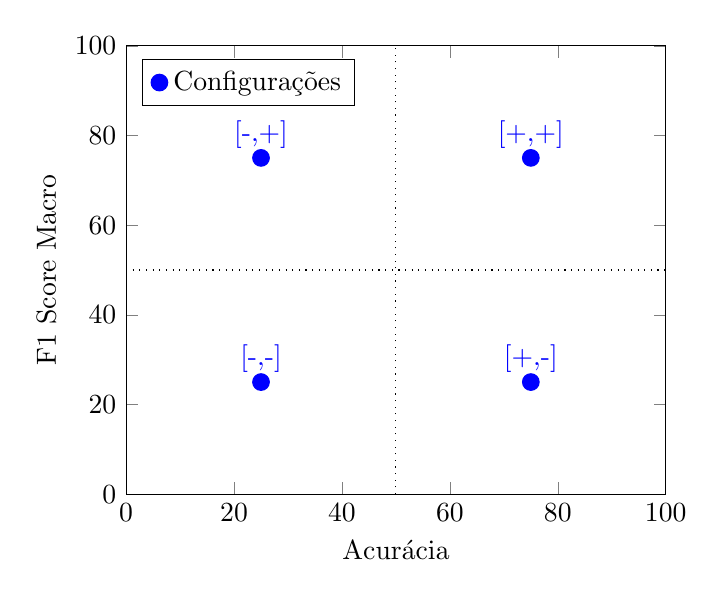
\begin{tikzpicture}
    \begin{axis}[
        xlabel={Acurácia},
        ylabel={F1 Score Macro},
        xmin=0, xmax=100,
        ymin=0, ymax=100,
        xtick={0,20,40,60,80,100},
        ytick={0,20,40,60,80,100},
        legend pos=north west,
        grid style=dashed,
    ]
    
    \draw[dotted] (50,0) -- (50,100);
    \draw[dotted] (0,50) -- (100,50);
    
    \addplot[
        only marks,
        mark=*,
        blue,
        mark options={scale=1.5},
        nodes near coords,
        point meta=explicit symbolic,
    ] table[meta=label] {
    x y label
    25 75 [-,+]
    75 75 [+,+]
    25 25 [-,-]
    75 25 [+,-]
    };
    \legend{Configurações}
    \end{axis}
    \end{tikzpicture}
\caption{Interpretação do gráfico de dispersão relacionando acurácia e F1 Score Macro das combinações Argmax.}
    \label{fig:scatter_acuracia_f1score_ilustracao}
\end{figure}

No gráfico \ref{fig:scatter_acuracia_f1score} apresenta-se os métodos de maneira combinada.  Isto permite separar os métodos em quatro grupos distintos de configurações, divididos conforme a mediana de cada métrica. 

\begin{itemize}
    \item \textbf{Quadrante Superior Direito (++)}: Configurações com alto desempenho tanto em acurácia quanto em F1 Score Macro.
    \begin{itemize}
        \item Binary [1, 2] \& None: Acurácia = 89.56\%, F1 Score Macro = 70.09\%.
        \item TermFrequency [1, 2] \& L2: Acurácia = 79.65\%, F1 Score Macro = 55.56\%.
        \item TFIDF [1, 2] \& L2: Acurácia = 82.76\%, F1 Score Macro = 59.83\%.
        \item Binary [1, 1] \& None: Acurácia = 75.31\%, F1 Score Macro = 58.77\%.
        \item TermFrequency [1, 1] \& L2: Acurácia = 77.05\%, F1 Score Macro = 52.31\%.
        \item TFIDF [1, 1] \& L2: Acurácia = 78.37\%, F1 Score Macro = 55.20\%.
    \end{itemize}

    \item \textbf{Quadrante Inferior Direito (+-)}: Configurações com alta acurácia mas F1 Score Macro abaixo de 50\%.
    \begin{itemize}
        \item TFIDF [1, 1] \& None: Acurácia = 70.64\%, F1 Score Macro = 32.10\%.
        \item TFIDF [1, 2] \& None: Acurácia = 74.57\%, F1 Score Macro = 37.67\%.
        \item TermFrequency [1, 1] \& None: Acurácia = 63.76\%, F1 Score Macro = 23.44\%.
        \item TermFrequency [1, 2] \& None: Acurácia = 66.68\%, F1 Score Macro = 27.08\%.
    \end{itemize}

    \item \textbf{Quadrante Inferior Esquerdo (--) }: Configurações com desempenho abaixo de 50\% em ambas as métricas.
    \begin{itemize}
        \item Binary [1, 1] \& L2: Acurácia = 19.07\%, F1 Score Macro = 25.39\%.
        \item Binary [1, 2] \& L2: Acurácia = 31.30\%, F1 Score Macro = 33.82\%.
    \end{itemize}

    \item \textbf{Quadrante Superior Esquerdo (-+)}: Não aplicável, pois não há configurações com acurácia < 50\% e F1 Score Macro >= 50\%.
\end{itemize}

Concluída a classificação preliminar das configurações por meio do método Argmax, a investigação avança para uma avaliação detalhada de cada técnica de classificação textual individualmente. Esta etapa visa avaliar o impacto dos parâmetros específicos — incluindo o método de vetorização, a aplicação de N-Gramas e a normalização — na acurácia e no F1 Score Macro associados a cada método.

\begin{figure}[H]
    \centering
    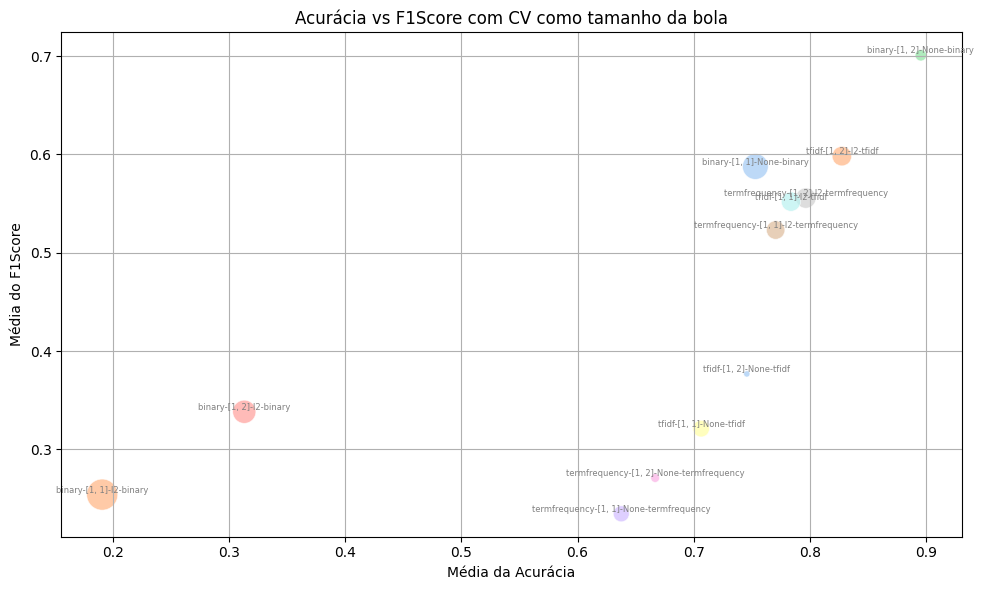
\includegraphics[width=0.8\textwidth]{images/ArgmaxScatterTodos.png}
    \caption{Gráfico de dispersão relacionando acurácia e F1 Score Macro das combinações Argmax.}
    \label{fig:scatter_acuracia_f1score}
\end{figure}

\subsection{Análise do Método Binário}

É avaliado as variações em relação ao N-Grama e Normalização.  Os resultados são apresentados na tabela \ref{tab:resultado_binario}.  Observando-a, a configuração binária sem normalização e com N-Gramas [1, 2] (binary-[1, 2]-None) apresentou o melhor desempenho, alcançando a maior média de acurácia (89.56\%) e F1 Score Macro (70.09\%). Em contraste, a configuração com normalização L2 e unigramas (binary-[1, 1]-l2) registrou o pior desempenho, com as menores médias de acurácia (19.07\%) e F1 Score Macro (25.39\%).

\begin{table}[H]
\centering
\caption{Resultados estatísticos dos testes para o método Argmax Binário}
\label{tab:resultado_binario}
\footnotesize % Diminui a fonte da tabela
\begin{tabular}{lllrrrrrr}
\hline
Método & NGram & Norm & \multicolumn{3}{c}{Acurácia (\%)} & \multicolumn{3}{c}{F1 Score Macro(\%)} \\
& & & Média & CV & \# & Média & CV & \# \\
\hline
Binary & [1, 1] & None & 75.31 & 0.44 & 2 & 58.77 & 3.15 & 2 \\
Binary & [1, 1] & L2 & 19.07 & 2.40 & 4 & 25.39 & 2.04 & 4 \\
Binary & [1, 2] & None & 89.56 & 0.21 & 1 & 70.09 & 1.91 & 1 \\
Binary & [1, 2] & L2 & 31.30 & 1.48 & 3 & 33.82 & 1.77 & 3 \\
\hline
\end{tabular}
\end{table}

Os boxplots, \ref{fig:boxplot_binary} indicam uma forte correlação entre a acurácia e o f1scoremacro, a dispersões são relativamente baixas. 
% Boxplot e Gráfico de Dispersão para o método Binary
\begin{figure}[H]
    \centering
    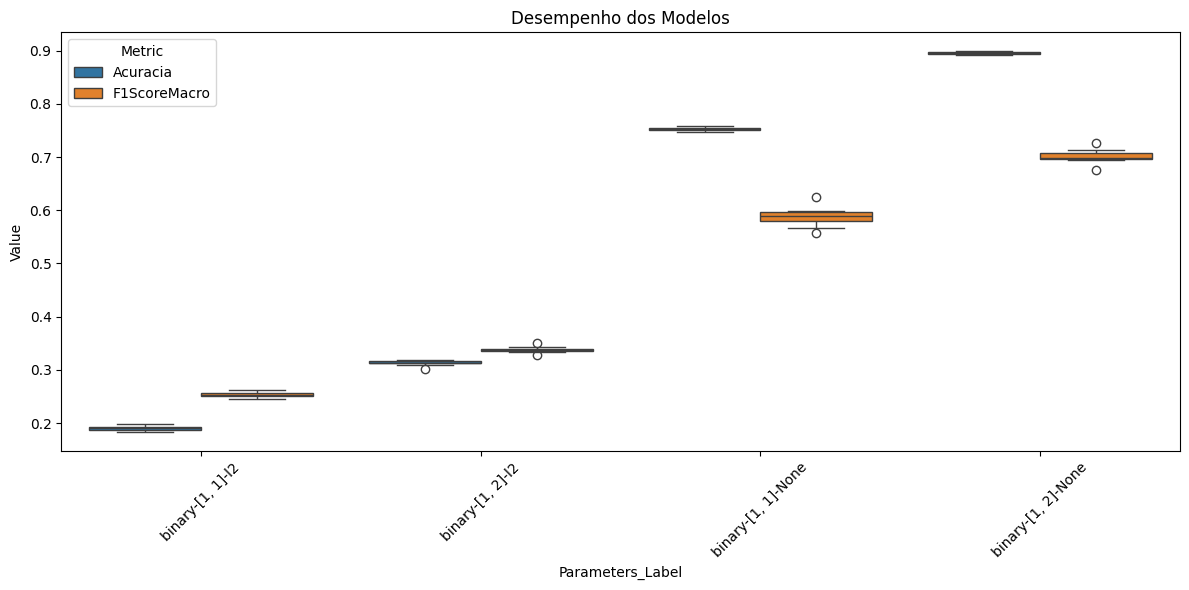
\includegraphics[width=0.8\textwidth]{images/boxbinario.png}
    \caption{Boxplot dos F1 Scores Macro das combinações Argmax para o método Binary.}
    \label{fig:boxplot_binary}
\end{figure}

O gráfico de dispersão, \ref{fig:scatter_acuracia_f1score_binary}, ilustra o impacto significativo dos parâmetros de normalização e range de N-Gramas no desempenho do modelo. Configurações sem normalização L2 tendem a agrupar-se no quadrante de desempenho superior, destacando a influência negativa da normalização L2 na classificação binária para este conjunto de dados.  É observável que ao se aplicar o ngram (1,2), as métricas melhoram, indicando melhoria no método.

\begin{figure}[H]
    \centering
    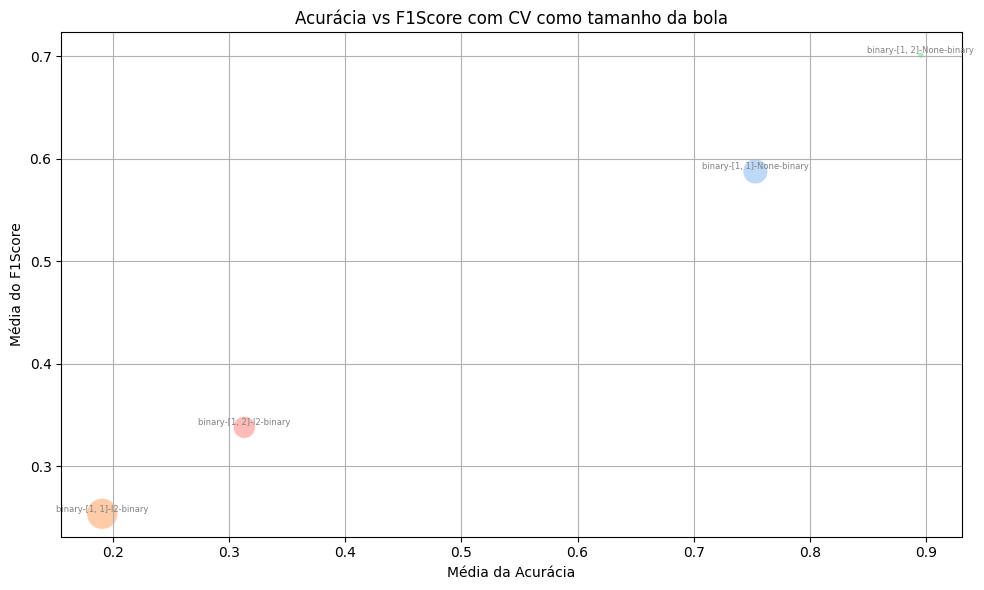
\includegraphics[width=0.8\textwidth]{images/dispersaobinario.png}
    \caption{Gráfico de dispersão relacionando acurácia e F1 Score Macro das combinações Argmax para o método Binary.}
    \label{fig:scatter_acuracia_f1score_binary}
\end{figure}

Em resumo, os resultados sugerem que a ausência de normalização L2, combinada com o uso de bigramas, otimiza significativamente o desempenho da classificação binária. Esse padrão pode ser atribuído à maior capacidade dos bigramas em capturar contextos relevantes sem a penalização da normalização.  É explicável que ao se normalizar um vetor binário, classes com mais termos tendem a possuir valores menores para o token, o que por sua vez perde relevância ao se realizar a avaliação da similaridade.

\subsection{Análise do Método TermFrequency}

A Tabela \ref{tab:resultadoargmaxtf_rankings} apresenta os resultados para o método tf.  Os resultados indicam que a configuração utilizando bigramas (NGram [1,2]) com aplicação de normalização L2 alcançou a melhor performance em ambos os indicadores. Especificamente, a configuração TermFrequency [1, 2] com L2 destacou-se, sugerindo que a inclusão de bigramas e a normalização são benéficas para a análise de textos curtos, ao capturar relações contextuais mais complexas e reduzir a influência de termos frequentes, respectivamente.

\begin{table}[H]
\centering
\caption{Resultados estatísticos dos testes para o método Argmax TF}
\label{tab:resultadoargmaxtf_rankings}
\footnotesize % Diminui a fonte da tabela
\begin{tabular}{lllrrrrrr}
\hline
Método & NGram & Norm & \multicolumn{3}{c}{Acurácia (\%)} & \multicolumn{3}{c}{F1 Score Macro(\%)} \\
& & & Média & CV & \# & Média & CV & \# \\
\hline
TermFrequency & [1, 1] & None & 63.76 & 0.41 & 4 & 23.44 & 2.05 & 4 \\
TermFrequency & [1, 1] & L2 & 77.05 & 0.24 & 2 & 52.31 & 2.46 & 2 \\
TermFrequency & [1, 2] & None & 66.68 & 0.28 & 3 & 27.08 & 1.69 & 3 \\
TermFrequency & [1, 2] & L2 & 79.65 & 0.29 & 1 & 55.56 & 2.61 & 1 \\
\hline
\end{tabular}
\end{table}

Os boxplots, \ref{fig:boxplot_tf}, associados a estas configurações ilustram uma variância reduzida nos resultados de acurácia e F1Score não normalizado.  Quando ocorre normalização a um leve aumenta da dispersão em relação ao F1Score. Novamente, a correlação entre os rankings de acurácia e F1 Score Macro reforça a ideia de que as configurações que performam bem em uma métrica tendem a performar bem na outra, demonstrando uma correlação em performar bem em uma métrica implica em performar bem em outra, medida global e medida interna.

\begin{figure}[H]
    \centering
    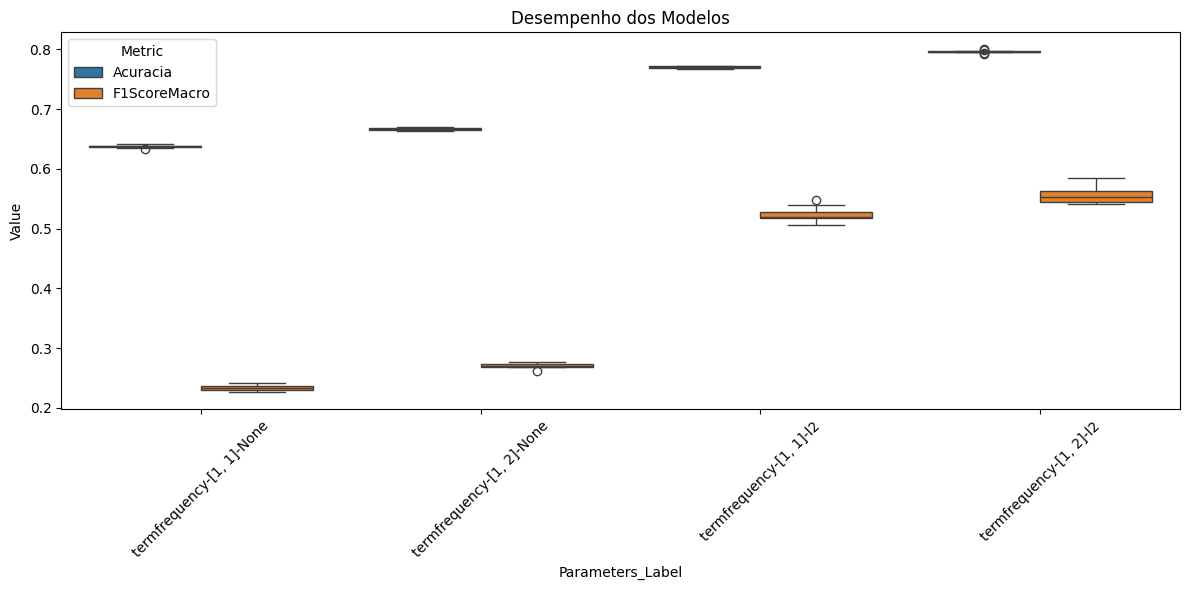
\includegraphics[width=0.8\textwidth]{images/boxtf.png}
    \caption{Boxplot dos F1 Scores Macro das combinações Argmax para o método TFIDF.}
    \label{fig:boxplot_tf}
\end{figure}

O gráfico de dispersão, \ref{fig:scatter_tf}, permite observar o maior ganho, quando aplicado sobre a normalização. 
 Por outro lado aumentar a quantidade de tokens não influencia de maneira significativa a performance do modelo.  A normalização incrementa significativamente a performance sobre a métrica F1Score, devido a tirar o efeito do desbalanceamento.  

\begin{figure}[H]
    \centering
    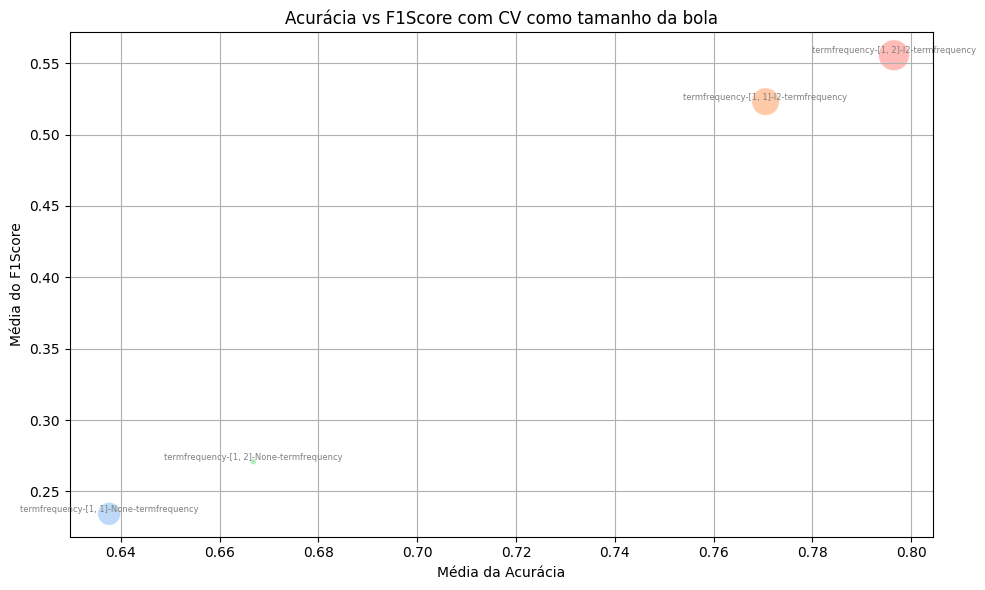
\includegraphics[width=0.8\textwidth]{images/dispersaotf.png}
    \caption{Gráfico de dispersão relacionando acurácia e F1 Score Macro das combinações Argmax para o método TFIDF.}
    \label{fig:scatter_tf}
\end{figure}

Em suma, a análise do método TF revela uma preferência clara pelas configurações que utilizam bigramas em conjunto com normalização L2. Sendo a normalização que apresenta o maior impacto.


\subsection{Análise do Método TFIDF}

A análise dos resultados obtidos pelo método TFIDF, conforme apresentado na Tabela \ref{tab:resultadoargmaxtfidf_rankings}, destaca que configuração TFIDF [1, 2] e L2 como a mais eficaz, alcançando a maior média tanto em acurácia (82.76\%) quanto em F1 Score Macro (59.83\%). Tal configuração sugere que a utilização de bigramas, ao adicionar uma camada de análise contextual, juntamente com a normalização L2, que penaliza termos excessivamente frequentes, cria um equilíbrio ideal para a captura de nuances linguísticas em textos curtos.

O impacto da normalização L2, em particular, merece destaque. Ao comparar as configurações com e sem normalização L2, observa-se uma melhoria consistente nos resultados quando a normalização é aplicada. Isso indica que a redução da influência de termos de alta frequência pode ser crucial para aumentar a eficácia da classificação, especialmente em conjuntos de dados onde a prevalência de certos termos pode distorcer a representação do texto.

\begin{table}[H]
\centering
\caption{Resultados estatísticos dos testes para o método TFIDF com diferentes configurações}
\label{tab:resultadoargmaxtfidf_rankings}
\footnotesize % Diminui a fonte da tabela
\begin{tabular}{lllrrrrrr}
\hline
Método & NGram & Norm & \multicolumn{3}{c}{Acurácia (\%)} & \multicolumn{3}{c}{F1 Score Macro(\%)} \\
& & & Média & CV & \# & Média & CV & \# \\
\hline
TFIDF & [1, 1] & None & 70.64 & 0.28 & 4 & 32.10 & 2.25 & 4 \\
TFIDF & [1, 1] & L2 & 78.37 & 0.32 & 3 & 55.20 & 2.47 & 3 \\
TFIDF & [1, 2] & None & 74.57 & 0.33 & 2 & 37.67 & 1.53 & 2 \\
TFIDF & [1, 2] & L2 & 82.76 & 0.29 & 1 & 59.83 & 2.52 & 1 \\
\hline
\end{tabular}
\end{table}

Os boxplots, \ref{fig:boxplot_tfidf} permite novamente verificar a correlação entre acurácia e f1score.  Além disto, percebe-se o impacto normalização sendo o mais impactante, promovendo tanto ganho em acurácia quando ganho em f1score.  Novamente o F1Score apreenta um ligeiro aumento de variabilidade quando se aplica a normalização, e por fim, o impacto do aumento de termos, ngram (1,2), melhora o desempenho, mas não na mesma intensidade que a normalização..


% Boxplot e Gráfico de Dispersão para o método TFIDF
\begin{figure}[H]
    \centering
    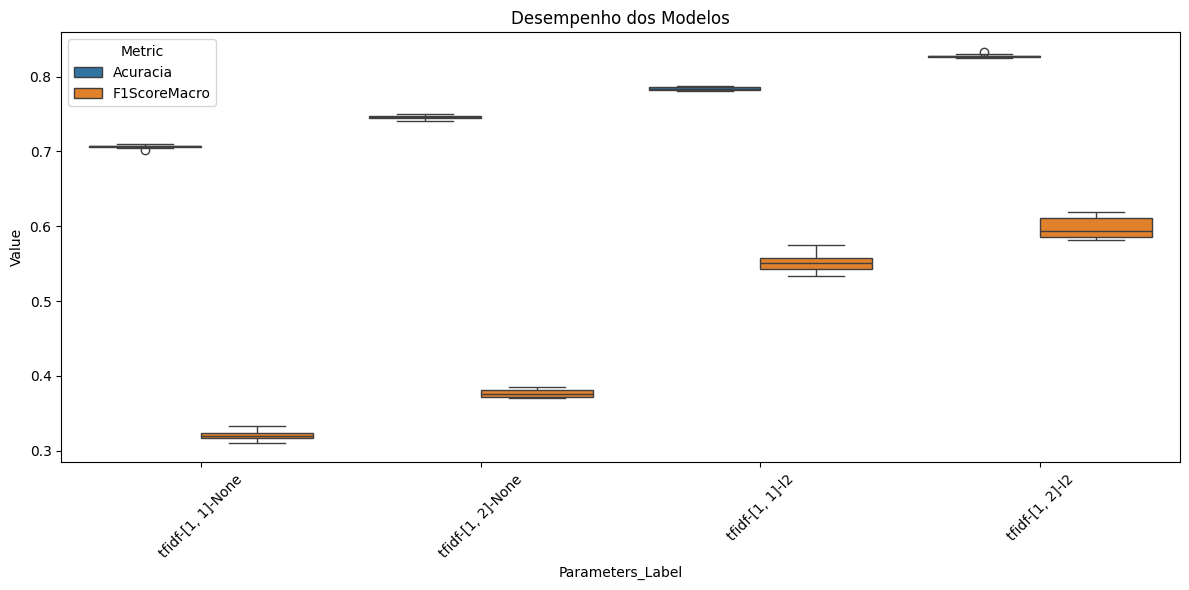
\includegraphics[width=0.8\textwidth]{images/boxtfidf.png}
    \caption{Boxplot dos F1 Scores Macro das combinações Argmax para o método TFIDF.}
    \label{fig:boxplot_tfidf}
\end{figure}

O gráfico de dispersão, \ref{fig:scatter_tfidf}, permite confirmar visualmente a análise acima de maneira combinda.  

\begin{figure}[H]
    \centering
    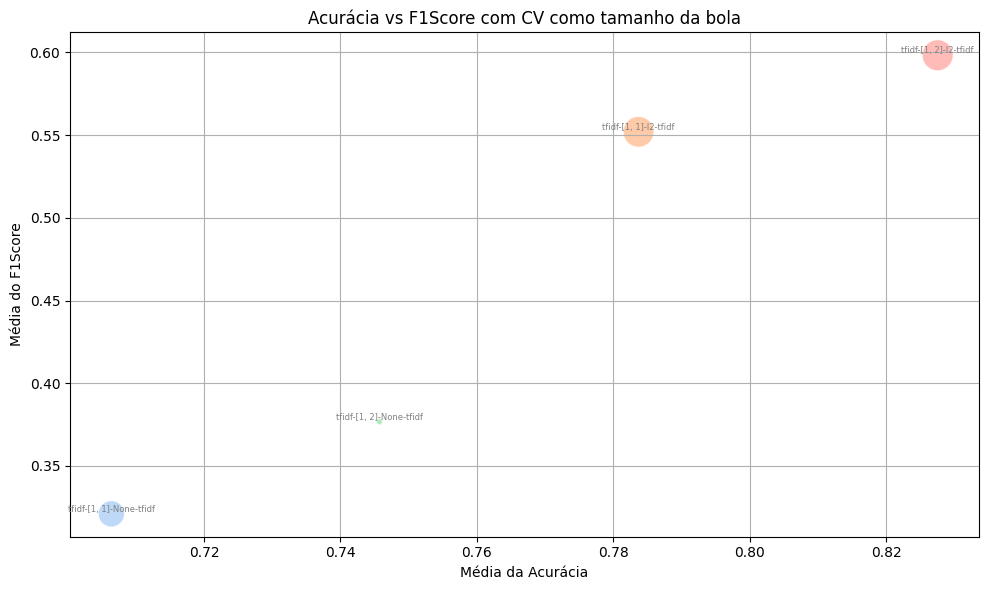
\includegraphics[width=0.8\textwidth]{images/dispersaotfidf.png}
    \caption{Gráfico de dispersão relacionando acurácia e F1 Score Macro das combinações Argmax para o método TFIDF.}
    \label{fig:scatter_tfidf}
\end{figure}

Em conclusão, a normalização L2 provoca a maior alteração nos resultados, seguido de uma melhora não tão significativa dada pela tokenização.


\subsection{Considerações Finais sobre Configurações Testadas}

Ao finalizar a avaliação das diversas configurações testadas para os métodos de classificação Argmax, emerge um panorama claro sobre a influência dos parâmetros de normalização e n-gram na eficácia da classificação de textos curtos. Esta seção visa sintetizar as conclusões extraídas das análises anteriores e discutir as implicações práticas destes achados.

A Tabela \ref{tab:resumo_parametros} apresenta os parâmetros sugeridos para cada modelo bem como o parâmetro que promove o maior impacto.

\begin{table}[H]
\centering
\caption{Parâmetros sugeridos para os métodos Argmax baseados em Acurácia e F1 Score Macro ($^*$ parâmetro mais impactante)}
\label{tab:resumo_parametros}
\begin{tabular}{lcc}
\hline
\textbf{Método} & \textbf{Normalização} & \textbf{N-Gram} \\
\hline
Binary & None$^*$ & [1, 2] \\
TermFrequency & L2$^*$ & [1, 2] \\
TFIDF & L2 & [1, 2]$^*$ \\
\hline
\end{tabular}
\end{table}

Neste segmento, são resumidos os principais achados decorrentes da avaliação das configurações testadas nos métodos de classificação Argmax, com ênfase na influência exercida pelos parâmetros de normalização e n-gram sobre a eficácia da classificação de textos curtos. Os padrões identificados nas preferências de configuração para cada método de classificação são delineados a seguir em forma de pontos-chave:

\begin{itemize}
    \item Para o método Binary:
    \begin{itemize}
        \item A ausência de normalização L2 foi determinante para alcançar melhores resultados, sugerindo que, no contexto binário, a normalização pode penalizar classes com uma diversidade maior de termos.
        \item A utilização de bigramas [1, 2] contribuiu para uma melhoria secundária, evidenciando que a presença ou ausência de termos constitui um fator impactante na classificação.
    \end{itemize}
    \item Para os métodos TermFrequency e TFIDF:
    \begin{itemize}
        \item A aplicação da normalização L2, em combinação com bigramas [1, 2], foi identificada como a configuração mais eficaz, sublinhando a importância da normalização para contrabalançar a influência de termos frequentes e da expansão contextual para enriquecer a representação textual.
        \item A normalização L2 assume um papel primordial no método TermFrequency, enquanto sua relevância é secundária no método TFIDF, o qual intrinsecamente ajusta a influência de termos frequentes através de sua formulação.
        \item A inclusão de bigramas [1, 2] melhorou o desempenho dos modelos, indicando que a captura de contexto adicional beneficia a classificação.
    \end{itemize}
\end{itemize}

\section{Definição de Novas Métricas de Desempenho}

Diante da necessidade de avaliar de maneira integrada o desempenho dos modelos de classificação, especialmente em contextos de classes desbalanceadas, propõe-se duas novas métricas: o Índice de Eficiência Geral (IEG) e o Índice de Eficiência Geral Estabilizada (IEGE). Estas métricas visam proporcionar uma avaliação unificada que considere tanto a acurácia quanto o F1 Score Macro, além da robustez do modelo, medida pelo Coeficiente de Variação (CV).  O objetivo das duas medidas é condensar o desempenho dos modelos tanto de maneira global, medido pela acurácio, tanto pelo desempenho pontual, medido pela F1ScoreMacro.  O segundo índice acrescenta uma ponderação em relação ao coeficiente de variação de forma a privilegiar modelos que mantenham sua capacidade de generalização mesmo sobre amostras diferentes.

\subsection{Índice de Eficiência Geral (IEG)}

O Índice de Eficiência Geral (IEG) é definido como a distância euclidiana entre a acurácia e o F1 Score Macro no espaço bidimensional, normalizado pela raiz quadrada de 2, para que os valores estejam entre 0 e 1. A equação para o IEG é dada por:

\begin{equation}
IEG = \frac{\sqrt{(Acuracia)^2 + (F1ScoreMacro)^2}}{\sqrt{2}}
\end{equation}

onde Acurácia e F1ScoreMacro são os valores decimais dessas métricas (isto é, valores percentuais divididos por 100).

\subsection{Índice de Eficiência Geral Estabilizada (IEGE)}

O Índice de Eficiência Geral Estabilizada (IEGE) expande o conceito do IEG ao incorporar um fator penalizador baseado no Coeficiente de Variação (CV) das métricas, refletindo a robustez do modelo. A equação para o IEGE é:

\begin{equation}
IEE-Stab = \frac{\sqrt{(Acurácia \cdot (1 - CV))^2 + (F1ScoreMacro \cdot (1 - CV))^2}}{\sqrt{2}}
\end{equation}

Assim, o IEGE não apenas mede o desempenho do modelo em termos de acurácia e F1 Score Macro, mas também ajusta esses valores com base na consistência do modelo, oferecendo uma perspectiva mais abrangente sobre sua eficácia e confiabilidade.

Estas métricas foram aplicadas aos resultados obtidos com diferentes configurações dos métodos de classificação Argmax, permitindo uma comparação direta entre eles, considerando não só o desempenho, mas também a estabilidade dos modelos em diferentes execuções.

\subsubsection{Aplicação e Resultados}

As métricas propostas foram aplicadas ao conjunto de variações dos métodos baseados em argmax, cujos resultados são apresentados na Tabela \ref{tab:Índice de Eficiência Geral (IEG) e Estabilizado (IEGE)}. Observa-se que essas métricas fornecem um índice unificado capaz de refletir eficientemente o desempenho dos métodos tanto em aspectos gerais quanto específicos. Notavelmente, a análise revela uma similaridade nos resultados entre o IEG e o IEGE, o que pode ser atribuído à pouca variação nos coeficientes de variação entre os diferentes métodos avaliados. Essa característica sublinha a possibilidade de classificar os métodos desde a melhor até a pior configuração de maneira consistente, corroborando os resultados observados em diversas representações gráficas neste estudo.

\begin{table}[H]
\centering
\caption{Índice de Eficiência Geral (IEG) e Estabilizado (IEGE)}
\label{tab:Índice de Eficiência Geral (IEG) e Estabilizado (IEGE)}
\footnotesize % Diminui a fonte da tabela
\begin{tabular}{lllrrrrrrrrrr}
\hline
Método & NGram & Norm & \multicolumn{3}{c}{Acurácia (\%)} & \multicolumn{3}{c}{F1 Score Macro (\%)} & \multicolumn{2}{c}{IEG} & \multicolumn{2}{c}{IEGE} \\
& & & Média & CV & \# & Média & CV & \# & Valor & Rank & Valor & Rank \\
\hline
Binary & [1, 2] & None & 89.56 & 0.21 & 1 & 70.09 & 1.91 & 1 & 80.4 & 1 & 79.7 & 1 \\
TFIDF & [1, 2] & L2 & 82.76 & 0.29 & 2 & 59.83 & 2.52 & 2 & 72.2 & 2 & 71.5 & 2 \\
TF & [1, 2] & L2 & 79.65 & 0.29 & 3 & 55.56 & 2.61 & 4 & 68.7 & 3 & 68.0 & 3 \\
TFIDF & [1, 1] & L2 & 78.37 & 0.32 & 5 & 55.20 & 2.47 & 6 & 67.8 & 4 & 67.1 & 4 \\
Binary & [1, 1] & None & 75.31 & 0.44 & 6 & 58.77 & 3.15 & 3 & 67.5 & 5 & 66.6 & 5 \\
TF & [1, 1] & L2 & 77.05 & 0.24 & 4 & 52.31 & 2.46 & 5 & 65.9 & 6 & 65.2 & 6 \\
TFIDF & [1, 2] & None & 74.57 & 0.33 & 7 & 37.67 & 1.53 & 7 & 59.1 & 7 & 58.7 & 7 \\
TFIDF & [1, 1] & None & 70.64 & 0.28 & 8 & 32.10 & 2.25 & 9 & 54.9 & 8 & 54.5 & 8 \\
TF & [1, 2] & None & 66.68 & 0.28 & 9 & 27.08 & 1.69 & 10 & 50.9 & 9 & 50.6 & 9 \\
TF & [1, 1] & None & 63.76 & 0.41 & 10 & 23.44 & 2.05 & 12 & 48.0 & 10 & 47.7 & 10 \\
Binary & [1, 2] & L2 & 31.30 & 1.48 & 11 & 33.82 & 1.77 & 8 & 32.6 & 11 & 32.1 & 11 \\
Binary & [1, 1] & L2 & 19.07 & 2.40 & 12 & 25.39 & 2.04 & 11 & 22.5 & 12 & 22.0 & 12 \\
\hline
\end{tabular}
\end{table}




% % Repita a estrutura acima para cada método de ML analisado
% % Exemplo para um método de ML: SVM
% \section{Análise dos Resultados do Método SVM}
% \subsection{Resultado Geral}
% \subsubsection{Box Plot}
% \subsubsection{Tabela de Desempenho}
% \subsubsection{Análise ANOVA}

% \subsection{Impacto do Método de Vetorização}
% \subsubsection{Box Plot}
% \subsubsection{Tabela de Desempenho}
% \subsubsection{Análise ANOVA}

% \subsection{Impacto da Tokenização}
% \subsubsection{Box Plot}
% \subsubsection{Tabela de Desempenho}
% \subsubsection{Análise ANOVA}

% \subsection{Impacto da Normalização}
% \subsubsection{Box Plot}
% \subsubsection{Tabela de Desempenho}
% \subsubsection{Análise ANOVA}

% \subsection{Discussão dos Resultados do SVM}
% Discussão detalhada dos resultados obtidos com o método SVM, fazendo conexões com estudos anteriores e teorias relevantes.

% % Adicione seções similares para outros métodos de ML aqui

% \section{Resultado Geral Comparativo}
% Esta seção compara os resultados obtidos de todos os métodos analisados, destacando as principais diferenças e semelhanças em termos de desempenho.

% \subsection{Box Plots Comparativos}
% \subsection{Tabelas de Desempenho Comparativas}
% \subsection{Análise ANOVA Geral}

% \section{Considerações sobre os Resultados}
% Discussão sobre as limitações dos resultados, possíveis viéses e sugestões para pesquisas futuras.

% \section{Conclusões da Seção de Resultados}
% Sumário dos achados mais significativos desta seção, reiterando a contribuição dos resultados para os objetivos da pesquisa.